\documentclass[tikz,border=2pt]{standalone}
\begin{document}
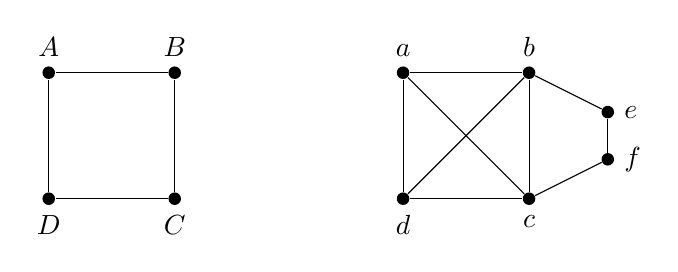
\begin{tikzpicture}[vertex/.style={circle,fill,inner sep=1.6pt}]
    % Grafo M
    \node[vertex,label=above:$A$] (A) at (0,1.6) {};
    \node[vertex,label=above:$B$] (B) at (1.6,1.6) {};
    \node[vertex,label=below:$D$] (D) at (0,0) {};
    \node[vertex,label=below:$C$] (C) at (1.6,0) {};
    \draw (A) -- (B);
    \draw (B) -- (C);
    \draw (C) -- (D);
    \draw (D) -- (A);

    % Grafo N
    \node[vertex,label=above:$a$] (a) at (4.5,1.6) {};
    \node[vertex,label=above:$b$] (b) at (6.1,1.6) {};
    \node[vertex,label=below:$d$] (d) at (4.5,0) {};
    \node[vertex,label=below:$c$] (c) at (6.1,0) {};
    \node[vertex,label=right:$e$] (e) at (7.1,1.1) {};
    \node[vertex,label=right:$f$] (f) at (7.1,0.5) {};
    \draw (a) -- (b);
    \draw (a) -- (d);
    \draw (a) -- (c);
    \draw (b) -- (d);
    \draw (b) -- (c);
    \draw (d) -- (c);
    \draw (b) -- (e);
    \draw (e) -- (f);
    \draw (f) -- (c);
\end{tikzpicture}
\end{document}
